\documentclass[12pt]{article}
\usepackage[utf8]{inputenc}
\usepackage{graphicx} % Allows you to insert figures
\usepackage{subcaption}
\usepackage{amsmath} % Allows you to do equations
\usepackage{fancyhdr} % Formats the header
\usepackage{geometry} % Formats the paper size, orientation, and margins
\usepackage{dirtytalk} % typesetting different types of quotation
\usepackage[english]{babel}
\usepackage{csquotes}
\usepackage{hyperref}
\usepackage{listings}
\lstset{
    language=C,
    basicstyle=\ttfamily, 
    numberstyle=\tiny,
    basicstyle=\small,
    frame=single,
    breaklines=true,
    stepnumber=1,                   % the step between two line-numbers.        
    tabsize=2,                      % sets default tabsize to 2 spaces
    breaklines=true,                % sets automatic line breaking
    breakatwhitespace=true,         % sets if automatic breaks should only happen at whitespace
    title=pseudocode
}


\usepackage{biblatex}
\addbibresource{reffs.bib}

\linespread{1.25} % About 1.5 spacing in Word
\setlength{\parindent}{0.8cm} % No paragraph indents
\setlength{\parskip}{0em} % Paragraphs separated by one line
\renewcommand{\headrulewidth}{0pt} % Removes line in header
\geometry{a4paper, portrait, margin=1in}
\setlength{\headheight}{14.49998pt}

\begin{document}
\begin{titlepage}
   \begin{center}
    \textsc{\large Ministry of Education of Republic of Moldova}\\[0.5cm]
    \textsc{\large Technical University of Moldova}\\[0.5cm]
    \textsc{\large Faculty of Computers, Informatics and Microelectronics}\\[0.5cm]
    \textsc{\large Software Engineering Department}\\[1.2cm]
    
    \vspace{25 mm}
    
    \textsc{\Large Computer Programming}\\[0.5cm]
    \textsc{\large Laboratory work \#2}\\[0.5cm]    % <<<<<<< CHANGE LAB NUMBER HERE
    
    \newcommand{\HRule}{\rule{\linewidth}{0.5mm}}
    \vspace{10 mm}
    \HRule \\[0.4cm]
    { \LARGE \bfseries One-Dimensional Array Operations and Processing }\\[0.4cm] % <<<<<<< CHANGE LAB TITLE HERE
    \HRule \\[1.5cm]
    
    \vspace{10mm}
    
    \begin{minipage}[t]{0.4\textwidth}
    \begin{flushleft} \large
    \emph{Author:} \\
    Andrei \textsc{Chicu}\\                         % <<<<<<< CHANGE YOUR NAME HERE
    std. gr. FAF-233                                % <<<<<<< CHANGE GROUP NUMBER HERE
    \end{flushleft}
    \end{minipage}
    ~
    \begin{minipage}[t]{0.4\textwidth}
    \begin{flushright} \large
    \emph{Verified:} \\
    Alexandru \textsc{Furdui}\\
    \end{flushright}
    \end{minipage}\\[3cm]
    
    \vspace{5 mm}
    \large Chișinău 2023\\[0.5cm]
    
    \vfill
    \end{center}
\end{titlepage}

\setcounter{page}{2}
\pagestyle{fancy}
\fancyhf{}
\rhead{\thepage}
\lhead{FAF-233 Andrei Chicu; Laboratory Work №2}

% \section*{Introduction}
\section*{Theory Background}
A one-dimensional array, often simply referred to as an "array," is a data structure in computer programming that represents a collection of elements of the same data type stored in a linear sequence. These elements are typically accessed using an index or position within the array. One-dimensional arrays are among the simplest and most commonly used data structures in programming.
I have researched the following sorting algorithms in order to implement them, and compare their speed:
\begin{enumerate}
    \item Bubble sort
    \item Selection sort
    \item Insertion sort
    \item Quick sort
\end{enumerate}
And also, have learned the uses of pointers and their relation with arrays; to allocate\cite{malloc} memory and copy\cite{memcpy} an array to this memory and have relied on these functions:
\begin{enumerate}
    \item \texttt{malloc()}
    \item \texttt{memcpy()}
    \item \texttt{free()}
\end{enumerate}

\section*{The Task}

\textbf{2.3 Hard}\\
Implement these sorting algorithms\cite{geeks}
\begin{enumerate}
    \item Bubble
    \item Selection
    \item Insertion 
    \item Quick Sort
\end{enumerate}
and explain them.

\pagebreak
\section*{Technical implementation}
\begin{lstlisting}
FUNCTION print_arr(arr: Array of Integer, len: Integer, time: Double)
    IF time > 0 THEN
        PRINT "Time taken: " + time
    END IF
    FOR i FROM 0 TO len - 1 DO
        PRINT arr[i] + " "
    END FOR
    PRINT NEWLINE
END FUNCTION

FUNCTION swap(xp: Pointer to Integer, yp: Pointer to Integer)
    SET temp = *xp
    *xp = *yp
    *yp = temp
END FUNCTION

FUNCTION quick_sort_part(arr: Array of Integer, low: Integer, high: Integer) -> Integer
    SET pivot = arr[high]
    SET i = low - 1

    FOR j FROM low TO high - 1 DO
        IF arr[j] < pivot THEN
            INCREMENT i
            CALL swap(&arr[i], &arr[j])
        END IF
    END FOR

    CALL swap(&arr[i + 1], &arr[high])
    RETURN i + 1
END FUNCTION

FUNCTION copy_arr(arr: Array of Integer, len: Integer) -> Array of Integer
    DECLARE b as Array of Integer with length len
    COPY arr TO b
    RETURN b
END FUNCTION

FUNCTION bubble_sort(a: Array of Integer, len: Integer, cnt: Pointer to Double) -> Array of Integer
    SET a_copy = copy_arr(a, len)
    SET t_start = current_time()

    FOR i FROM 0 TO len - 1 DO
        FOR j FROM 0 TO len - 2 DO
            IF a_copy[j] > a_copy[j + 1] THEN
                CALL swap(&a_copy[j], &a_copy[j + 1])
            END IF
        END FOR
    END FOR

    SET t_end = current_time()
    SET *cnt = (t_end - t_start) / CLOCKS_PER_SEC
    RETURN a_copy
END FUNCTION

FUNCTION selection_sort(a: Array of Integer, len: Integer, cnt: Pointer to Double) -> Array of Integer
    SET min_idx

    SET a_copy = copy_arr(a, len)
    SET t_start = current_time()

    FOR i FROM 0 TO len - 2 DO
        SET min_idx = i
        FOR j FROM i + 1 TO len - 1 DO
            IF a_copy[j] < a_copy[min_idx] THEN
                SET min_idx = j
            END IF
        END FOR

        IF min_idx != i THEN
            CALL swap(&a_copy[min_idx], &a_copy[i])
        END IF
    END FOR

    SET t_end = current_time()
    SET *cnt = (t_end - t_start) / CLOCKS_PER_SEC
    RETURN a_copy
END FUNCTION

FUNCTION insertion_sort(a: Array of Integer, len: Integer, cnt: Pointer to Double) -> Array of Integer
    SET key, j, i

    SET a_copy = copy_arr(a, len)
    SET t_start = current_time()

    FOR i FROM 1 TO len - 1 DO
        SET key = a_copy[i]
        SET j = i - 1

        WHILE j >= 0 AND a_copy[j] > key DO
            SET a_copy[j + 1] = a_copy[j]
            DECREMENT j
        END WHILE

        SET a_copy[j + 1] = key
    END FOR

    SET t_end = current_time()
    SET *cnt = (t_end - t_start) / CLOCKS_PER_SEC
    RETURN a_copy
END FUNCTION

FUNCTION quick_sort(a: Array of Integer, low: Integer, high: Integer)
    IF low < high THEN
        SET pi = quick_sort_part(a, low, high)
        CALL quick_sort(a, low, pi - 1)
        CALL quick_sort(a, pi + 1, high)
    END IF
END FUNCTION

FUNCTION main()
    DECLARE len as Integer
    DECLARE cnt as Double
    SET cnt = 0

    INPUT len
    DECLARE arr as Array of Integer with length len

    FOR i FROM 0 TO len - 1 DO
        INPUT arr[i]
    END FOR

    SET bubble_arr = bubble_sort(arr, len, &cnt)
    PRINT "Bubble sort"
    CALL print_arr(bubble_arr, len, cnt)
    FREE bubble_arr

    SET insertion_arr = insertion_sort(arr, len, &cnt)
    PRINT "Insertion sort"
    CALL print_arr(insertion_arr, len, cnt)
    FREE insertion_arr

    SET a_copy = copy_arr(arr, len)
    SET t_start = current_time()
    CALL quick_sort(a_copy, 0, len - 1)
    SET t_end = current_time()
    SET cnt = (t_end - t_start) / CLOCKS_PER_SEC
    PRINT "Quick sort"
    CALL print_arr(a_copy, len, cnt)
    FREE a_copy

    SET selection_arr = selection_sort(arr, len, &cnt)
    PRINT "Selection sort"
    CALL print_arr(selection_arr, len, cnt)
    FREE selection_arr

    RETURN 0
END FUNCTION
\end{lstlisting}

\section*{Results}
\hspace{0.8cm}
I have provided the program with a random array with the use of the for cycle of the shell, and the \texttt{\$RANDOM} global variable.\cite{bash_rand}

I have obtained the following time of execution for the implemented algorithms:
\begin{enumerate}
    \item \textbf{Bubble sort} 0.000146 seconds
    \item \textbf{Selection sort} 0.000063 seconds
    \item \textbf{Insertion sort} 0.000032 seconds
    \item \textbf{Quick sort} 0.000029 seconds
\end{enumerate}

\begin{figure}[!h]
  \centering
  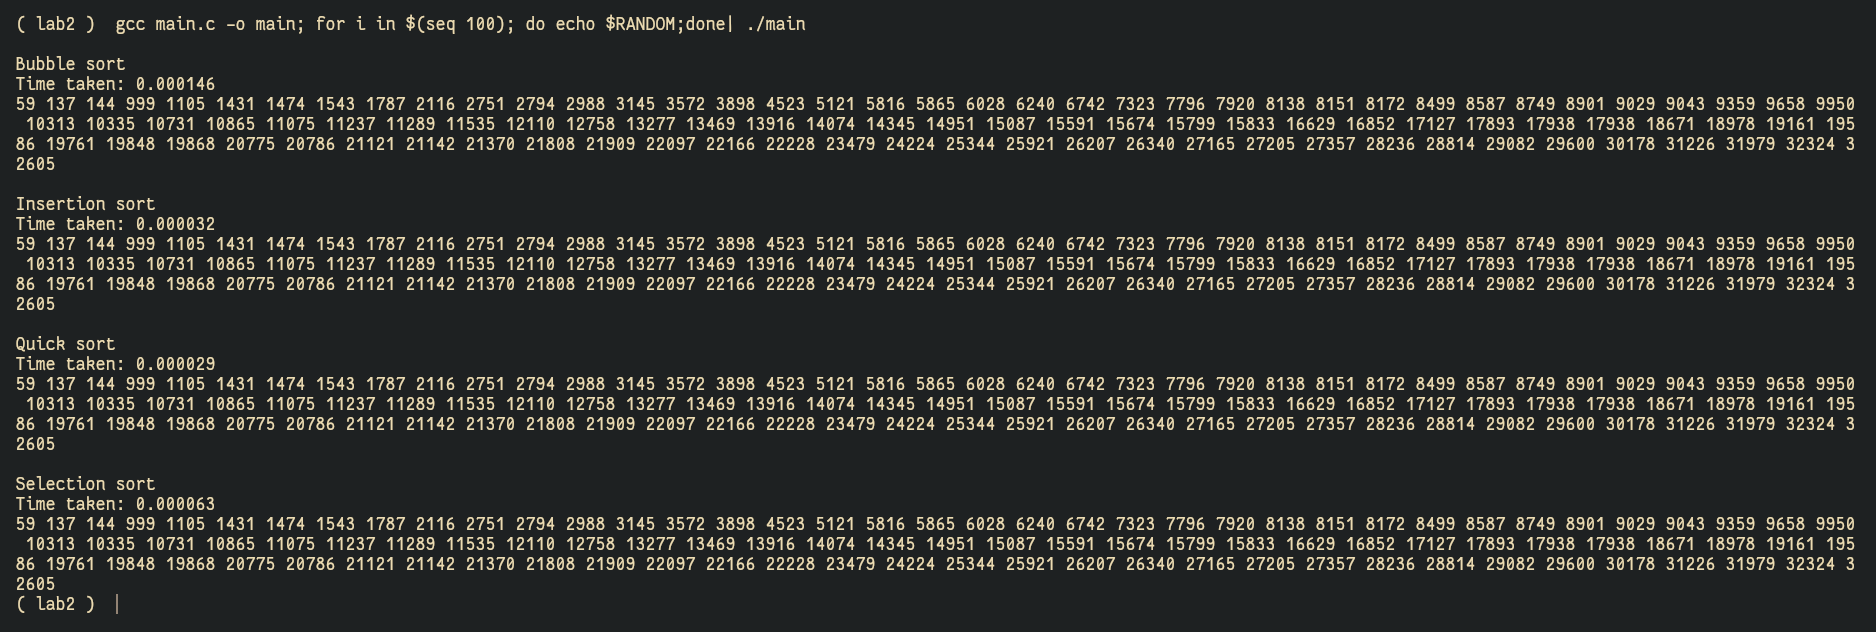
\includegraphics[width=\textwidth]{results.png}
  \caption{results}
\end{figure}


\section*{Conclusion}
\hspace{0.8cm}
In conclusion I can say that \textit{Quick sort} was on average the fastest of the algorithms, and bubble sort was the slowest.

But, interestingly enough, \textit{Insertion sort} was at times faster than \textit{Quick sort}, and the true difference of speed was seen only after several runs of the program  on different randomly generated arrays. This could imply that the randomly generated arrays were at times partially sorted, at which \textit{Insertion sort} performs well.\cite{etc}

\printbibliography
\end{document}
